\documentclass[a4paper]{article}
\usepackage{xcolor}
\usepackage{hyperref}
\usepackage[tightLists=false,hybrid=true]{markdown}
\usepackage{hyperref} % Required for adding links	and customizing them
\definecolor{linkcolour}{rgb}{0,0.2,0.6} % Link color
\hypersetup{colorlinks,breaklinks,urlcolor=linkcolour,linkcolor=linkcolour} % Set link colors throughout the document
\urlstyle{rm}


\usepackage[sc]{titlesec}
\titleformat{\section}{\Large\bfseries\sc\centering}{\thesection}{0em}{}
\titleformat{\subsection}{\Large\bfseries\sc\raggedright}{}{1em}{}
%\renewcommand{\thesubsection}{}
%\renewcommand{\thesection}{\arabic{section}}

\title{\textsc{\LARGE 2018 Work Log}\\ }
\date{}


\begin{document}
\maketitle


\section*{January}

\begin{markdown}
## Week 1

Returned from vacation in s.e. asia on Monday. I started working with easy maintenance tasks on my code.

- Created a git `development` to keep the `master` branch stable at all times.
- Polished up the `cmake` build script so that libraries are either found or fetched and installed properly in a platform independent way. Took some trial and error. 
- Added support for \href{www.travis-ci.com}{Travis-CI}, so that a `git push` now triggers a build in `g++-7.2` and `clang++-5.0`, and reports pass/fail on the github page.
- Added support for reading parameters from a text file instead of hard-coding them into a namespace .
- Rewrite routines for finding files in the filesystem, making better use of `<std::experimental::filesystem>` features for finding input and output files.

## Week 2

Continued on maintenance work. Almost finished

- Fixed some profiling issues. Timings were not clear enough.
- Fixed console output and implemented optional verbosity level, and optional timestamps.
- Started restructoring the algorithms using smart pointers everywhere, and using a Base class from which algorithms are derived (itebd, idmrg, fdmrg, etc). This modularization will speed up development time later, I believe.

## Week 3

- 


## Week 4
This week I started a new project: excited-state DMRG. I am supposed to implement SIMPS or xDMRG and then study the MBL transition shown in the picture.

\centering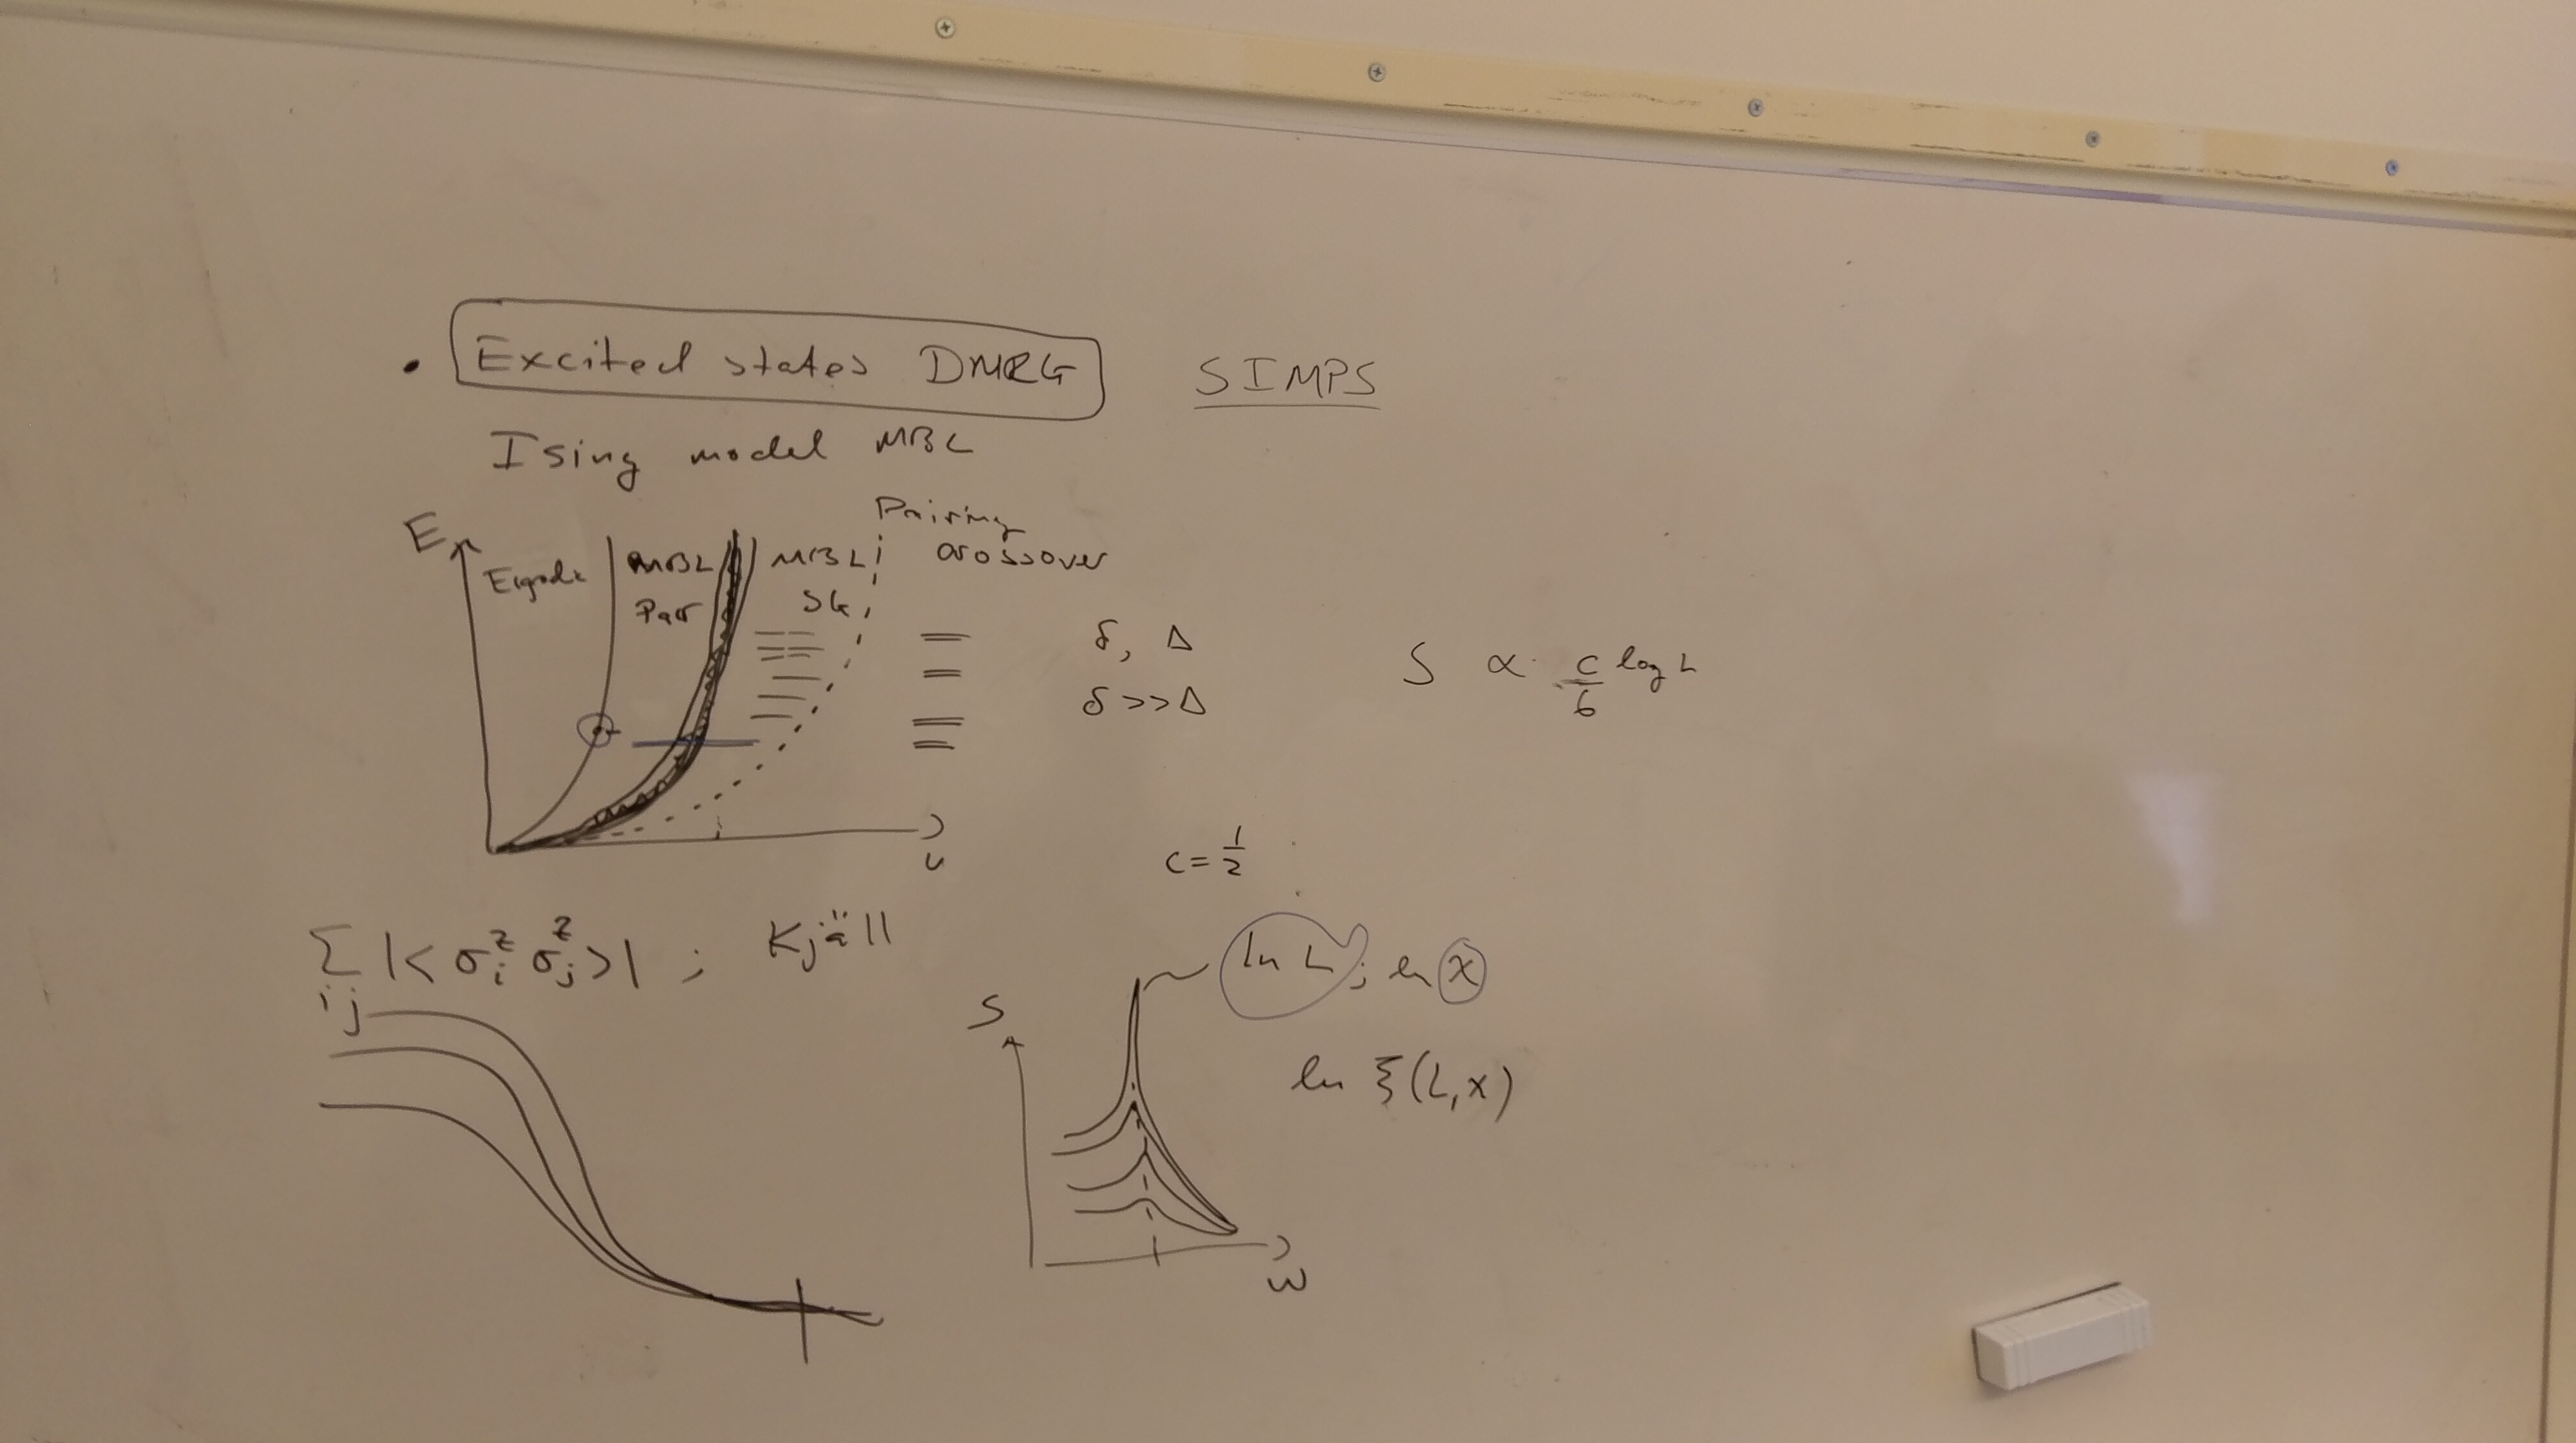
\includegraphics[width=0.9\textwidth, trim=12cm 2cm 40cm 12cm,clip]{figures/mblproject.jpg}

Other than that I continued the modularization, refactoring code. I'm trying to finish this as quickly as possible.

\end{markdown}

\section*{February}

\begin{markdown}
## Week 1
- Finished modularization. 
- Made another attempt to get Arpackc++ working to get eigenvalues of complex matrices. It worked! 
- Added the excited states module and started working on that.

## Week 2

- Changed the whole codebase to use complex numbers throughout. Having this double - complex switch is just messy, when complex numbers is ``lingua franca'' for MPS. 
- The xDMRG procedure is quite simple! Simply find all eigenvectors to the local effective hamiltonian,  i.e. $L-H-L$, where $H$ is an MPO, and chose the eigenvector with greatest overlap to the current state. Starting with a randomly oriented spin chain this converges usually to a highly excited state. Unfortunalely it doesn't let us target a specific energy, but perhaps if we use SIMPS in the beginning to target a specific part of the spectrum, we can then use xDMRG later to pinpoint a particular eigenstate in that region.

## Week 3

- To gauge how close the algorithm is to an eigenstate, I returned to the issue of computing the variance $\langle \Delta H \rangle = \langle H^2 \rangle - \langle H \rangle^2$. The method by C.West using characteristic functions seems very promising... if I could just get it to work. 

## Week 4

- Continued working on variances. 
- During the group meeting on Friday, a very fundamental error was pointed out to me. Essentially I hadn't been applying the unitary gates correctly; I applied them all, and then swapped. I am supposed to swap between every gate, and only then is a singla ``tebd'' step complete. It is amazing that I've gotten correct results all  this time despite this flaw. 


\end{markdown}
\section*{March}
\begin{markdown}
- The variance method by C.West works, almost. There is a discrepancy compared to the ``double MPO - double environment'' method I use for DMRG. Now I need to compute the variance using the regular method with the normal 2-site Hamiltonians. Turns out this is quite difficult, because the infinite number of crossterms need to be summed over. There are two places where this is described:

	- Zauner-Stauber, V., Vanderstraeten, L., Fishman, M. T., Verstraete, F., \& Haegeman, J. (2017). \href{https://doi.org/10.1103/PhysRevB.97.045145}{Variational optimization algorithms for uniform matrix product states} 
	
	- Vanderstraeten, L. (n.d.). \href{http://quantumtensor.pks.mpg.de/wp-content/uploads/2016/06/notes_2.pdf}{Tangent space methods for matrix product states}




\end{markdown}


\end{document}